\documentclass[twoside]{book}

% Packages required by doxygen
\usepackage{calc}
\usepackage{doxygen}
\usepackage{graphicx}
\usepackage[utf8]{inputenc}
\usepackage{makeidx}
\usepackage{multicol}
\usepackage{multirow}
\usepackage{fixltx2e}
\PassOptionsToPackage{warn}{textcomp}
\usepackage{textcomp}
\usepackage[nointegrals]{wasysym}
\usepackage[table]{xcolor}

% NLS support packages
\usepackage{polski}
\usepackage[T1]{fontenc}

% Font selection
\usepackage[T1]{fontenc}
\usepackage{mathptmx}
\usepackage[scaled=.90]{helvet}
\usepackage{courier}
\usepackage{amssymb}
\usepackage{sectsty}
\renewcommand{\familydefault}{\sfdefault}
\allsectionsfont{%
  \fontseries{bc}\selectfont%
  \color{darkgray}%
}
\renewcommand{\DoxyLabelFont}{%
  \fontseries{bc}\selectfont%
  \color{darkgray}%
}
\newcommand{\+}{\discretionary{\mbox{\scriptsize$\hookleftarrow$}}{}{}}

% Page & text layout
\usepackage{geometry}
\geometry{%
  a4paper,%
  top=2.5cm,%
  bottom=2.5cm,%
  left=2.5cm,%
  right=2.5cm%
}
\tolerance=750
\hfuzz=15pt
\hbadness=750
\setlength{\emergencystretch}{15pt}
\setlength{\parindent}{0cm}
\setlength{\parskip}{0.2cm}
\makeatletter
\renewcommand{\paragraph}{%
  \@startsection{paragraph}{4}{0ex}{-1.0ex}{1.0ex}{%
    \normalfont\normalsize\bfseries\SS@parafont%
  }%
}
\renewcommand{\subparagraph}{%
  \@startsection{subparagraph}{5}{0ex}{-1.0ex}{1.0ex}{%
    \normalfont\normalsize\bfseries\SS@subparafont%
  }%
}
\makeatother

% Headers & footers
\usepackage{fancyhdr}
\pagestyle{fancyplain}
\fancyhead[LE]{\fancyplain{}{\bfseries\thepage}}
\fancyhead[CE]{\fancyplain{}{}}
\fancyhead[RE]{\fancyplain{}{\bfseries\leftmark}}
\fancyhead[LO]{\fancyplain{}{\bfseries\rightmark}}
\fancyhead[CO]{\fancyplain{}{}}
\fancyhead[RO]{\fancyplain{}{\bfseries\thepage}}
\fancyfoot[LE]{\fancyplain{}{}}
\fancyfoot[CE]{\fancyplain{}{}}
\fancyfoot[RE]{\fancyplain{}{\bfseries\scriptsize Wygenerowano N, 14 cze 2015 11\+:27\+:40 dla Snakes, snakes programem Doxygen }}
\fancyfoot[LO]{\fancyplain{}{\bfseries\scriptsize Wygenerowano N, 14 cze 2015 11\+:27\+:40 dla Snakes, snakes programem Doxygen }}
\fancyfoot[CO]{\fancyplain{}{}}
\fancyfoot[RO]{\fancyplain{}{}}
\renewcommand{\footrulewidth}{0.4pt}
\renewcommand{\chaptermark}[1]{%
  \markboth{#1}{}%
}
\renewcommand{\sectionmark}[1]{%
  \markright{\thesection\ #1}%
}

% Indices & bibliography
\usepackage{natbib}
\usepackage[titles]{tocloft}
\setcounter{tocdepth}{3}
\setcounter{secnumdepth}{5}
\makeindex

% Hyperlinks (required, but should be loaded last)
\usepackage{ifpdf}
\ifpdf
  \usepackage[pdftex,pagebackref=true]{hyperref}
\else
  \usepackage[ps2pdf,pagebackref=true]{hyperref}
\fi
\hypersetup{%
  colorlinks=true,%
  linkcolor=blue,%
  citecolor=blue,%
  unicode%
}

% Custom commands
\newcommand{\clearemptydoublepage}{%
  \newpage{\pagestyle{empty}\cleardoublepage}%
}


%===== C O N T E N T S =====

\begin{document}

% Titlepage & ToC
\hypersetup{pageanchor=false,
             bookmarks=true,
             bookmarksnumbered=true,
             pdfencoding=unicode
            }
\pagenumbering{roman}
\begin{titlepage}
\vspace*{7cm}
\begin{center}%
{\Large Snakes, snakes }\\
\vspace*{1cm}
{\large Wygenerowano przez Doxygen 1.8.7}\\
\vspace*{0.5cm}
{\small N, 14 cze 2015 11:27:40}\\
\end{center}
\end{titlepage}
\clearemptydoublepage
\tableofcontents
\clearemptydoublepage
\pagenumbering{arabic}
\hypersetup{pageanchor=true}

%--- Begin generated contents ---
\chapter{Indeks hierarchiczny}
\section{Hierarchia klas}
Ta lista dziedziczenia posortowana jest z grubsza, choć nie całkowicie, alfabetycznie\+:\begin{DoxyCompactList}
\item \contentsline{section}{Algorithm}{\pageref{class_algorithm}}{}
\item \contentsline{section}{Data\+Manager}{\pageref{class_data_manager}}{}
\item \contentsline{section}{File\+Manager}{\pageref{class_file_manager}}{}
\item \contentsline{section}{I\+File}{\pageref{class_i_file}}{}
\begin{DoxyCompactList}
\item \contentsline{section}{File}{\pageref{class_file}}{}
\begin{DoxyCompactList}
\item \contentsline{section}{Algorithm\+File}{\pageref{class_algorithm_file}}{}
\item \contentsline{section}{Series\+File}{\pageref{class_series_file}}{}
\end{DoxyCompactList}
\end{DoxyCompactList}
\item \contentsline{section}{I\+Interpreter}{\pageref{class_i_interpreter}}{}
\begin{DoxyCompactList}
\item \contentsline{section}{Python\+Interpreter}{\pageref{class_python_interpreter}}{}
\end{DoxyCompactList}
\item \contentsline{section}{Point}{\pageref{class_point}}{}
\item \contentsline{section}{Series}{\pageref{class_series}}{}
\end{DoxyCompactList}

\chapter{Indeks klas}
\section{Lista klas}
Tutaj znajdują się klasy, struktury, unie i interfejsy wraz z ich krótkimi opisami\+:\begin{DoxyCompactList}
\item\contentsline{section}{\hyperlink{class_algorithm}{Algorithm} \\*Klasa \hyperlink{class_algorithm}{Algorithm} -\/ obiekty tej klasy przechowują informacje o algorytmach }{\pageref{class_algorithm}}{}
\item\contentsline{section}{\hyperlink{class_algorithm_file}{Algorithm\+File} \\*Klasa \hyperlink{class_algorithm_file}{Algorithm\+File} -\/ obiekty tej klasy przechowują informacje o pliku z którego jest wczytywany algorytm }{\pageref{class_algorithm_file}}{}
\item\contentsline{section}{\hyperlink{class_data_manager}{Data\+Manager} \\*Klasa \hyperlink{class_data_manager}{Data\+Manager} -\/ obiekt tej klasy zarządza przetwarzanymi w programie danymi, tj. algorytmami i seriami }{\pageref{class_data_manager}}{}
\item\contentsline{section}{\hyperlink{class_file}{File} \\*Klasa \hyperlink{class_file}{File} -\/ obiekty tej klasy przechowują informacje o pliku z którego są wczytywane dane }{\pageref{class_file}}{}
\item\contentsline{section}{\hyperlink{class_file_manager}{File\+Manager} \\*Klasa \hyperlink{class_file_manager}{File\+Manager} -\/ obiekt tej klasy służy do obsługi plików wczytywanych do programu }{\pageref{class_file_manager}}{}
\item\contentsline{section}{\hyperlink{class_i_file}{I\+File} \\*Klasa \hyperlink{class_i_file}{I\+File} -\/ interfejs dla różnych plików }{\pageref{class_i_file}}{}
\item\contentsline{section}{\hyperlink{class_i_interpreter}{I\+Interpreter} \\*Klasa \hyperlink{class_i_interpreter}{I\+Interpreter} -\/ interfejs dla interpreterów }{\pageref{class_i_interpreter}}{}
\item\contentsline{section}{\hyperlink{class_point}{Point} \\*Klasa \hyperlink{class_point}{Point} -\/ obiekty tej klasy przechowują informacje o punkcie serii }{\pageref{class_point}}{}
\item\contentsline{section}{\hyperlink{class_python_interpreter}{Python\+Interpreter} \\*Klasa \hyperlink{class_python_interpreter}{Python\+Interpreter} -\/ interpreter }{\pageref{class_python_interpreter}}{}
\item\contentsline{section}{\hyperlink{class_series}{Series} \\*Klasa \hyperlink{class_series}{Series} -\/ obiekt tej klasy przechowuje informacje o serii }{\pageref{class_series}}{}
\item\contentsline{section}{\hyperlink{class_series_file}{Series\+File} \\*Klasa \hyperlink{class_series_file}{Series\+File} -\/ obiekty tej klasy przechowują informacje o pliku z którego jest wczytywana seria }{\pageref{class_series_file}}{}
\end{DoxyCompactList}

\chapter{Dokumentacja klas}
\hypertarget{class_algorithm}{\section{Dokumentacja klasy Algorithm}
\label{class_algorithm}\index{Algorithm@{Algorithm}}
}


Klasa \hyperlink{class_algorithm}{Algorithm} -\/ obiekty tej klasy przechowują informacje o algorytmach.  




{\ttfamily \#include $<$algorithm.\+h$>$}

\subsection*{Metody publiczne}
\begin{DoxyCompactItemize}
\item 
Q\+String \hyperlink{class_algorithm_a5cd4793c1caa46a89884fcf1c92e5677}{get\+Name} ()
\begin{DoxyCompactList}\small\item\em get\+Name -\/ metoda pobiera nazwę algorytmu \end{DoxyCompactList}\item 
void \hyperlink{class_algorithm_a68542c56278158175c3d25f2e9325f89}{set\+Name} (Q\+String \+\_\+name)
\begin{DoxyCompactList}\small\item\em set\+Name -\/ metoda ustawia nazwę algorytmu \end{DoxyCompactList}\item 
Q\+String \hyperlink{class_algorithm_a8b5ecdf1f5be5996d77a5939622f7ca4}{get\+Script} ()
\begin{DoxyCompactList}\small\item\em get\+Script -\/ metoda pobiera skrypt do wykonania \end{DoxyCompactList}\item 
void \hyperlink{class_algorithm_a7d15e1a191268e75c249129da8787dc1}{set\+Script} (Q\+String \+\_\+script)
\begin{DoxyCompactList}\small\item\em set\+Script -\/ metoda ustawia skrypt algorytmu \end{DoxyCompactList}\end{DoxyCompactItemize}


\subsection{Opis szczegółowy}
Klasa \hyperlink{class_algorithm}{Algorithm} -\/ obiekty tej klasy przechowują informacje o algorytmach. 

\subsection{Dokumentacja funkcji składowych}
\hypertarget{class_algorithm_a5cd4793c1caa46a89884fcf1c92e5677}{\index{Algorithm@{Algorithm}!get\+Name@{get\+Name}}
\index{get\+Name@{get\+Name}!Algorithm@{Algorithm}}
\subsubsection[{get\+Name}]{\setlength{\rightskip}{0pt plus 5cm}Q\+String Algorithm\+::get\+Name (
\begin{DoxyParamCaption}
{}
\end{DoxyParamCaption}
)}}\label{class_algorithm_a5cd4793c1caa46a89884fcf1c92e5677}


get\+Name -\/ metoda pobiera nazwę algorytmu 

\begin{DoxyReturn}{Zwraca}
-\/ nazwa algorytmu 
\end{DoxyReturn}
\hypertarget{class_algorithm_a8b5ecdf1f5be5996d77a5939622f7ca4}{\index{Algorithm@{Algorithm}!get\+Script@{get\+Script}}
\index{get\+Script@{get\+Script}!Algorithm@{Algorithm}}
\subsubsection[{get\+Script}]{\setlength{\rightskip}{0pt plus 5cm}Q\+String Algorithm\+::get\+Script (
\begin{DoxyParamCaption}
{}
\end{DoxyParamCaption}
)}}\label{class_algorithm_a8b5ecdf1f5be5996d77a5939622f7ca4}


get\+Script -\/ metoda pobiera skrypt do wykonania 

\begin{DoxyReturn}{Zwraca}
-\/ skrpyt 
\end{DoxyReturn}
\hypertarget{class_algorithm_a68542c56278158175c3d25f2e9325f89}{\index{Algorithm@{Algorithm}!set\+Name@{set\+Name}}
\index{set\+Name@{set\+Name}!Algorithm@{Algorithm}}
\subsubsection[{set\+Name}]{\setlength{\rightskip}{0pt plus 5cm}void Algorithm\+::set\+Name (
\begin{DoxyParamCaption}
\item[{Q\+String}]{\+\_\+name}
\end{DoxyParamCaption}
)}}\label{class_algorithm_a68542c56278158175c3d25f2e9325f89}


set\+Name -\/ metoda ustawia nazwę algorytmu 


\begin{DoxyParams}{Parametry}
{\em \+\_\+name} & -\/ nazwa algorytmu do ustawienia \\
\hline
\end{DoxyParams}
\hypertarget{class_algorithm_a7d15e1a191268e75c249129da8787dc1}{\index{Algorithm@{Algorithm}!set\+Script@{set\+Script}}
\index{set\+Script@{set\+Script}!Algorithm@{Algorithm}}
\subsubsection[{set\+Script}]{\setlength{\rightskip}{0pt plus 5cm}void Algorithm\+::set\+Script (
\begin{DoxyParamCaption}
\item[{Q\+String}]{\+\_\+script}
\end{DoxyParamCaption}
)}}\label{class_algorithm_a7d15e1a191268e75c249129da8787dc1}


set\+Script -\/ metoda ustawia skrypt algorytmu 


\begin{DoxyParams}{Parametry}
{\em \+\_\+script} & -\/ skrypt do ustawienia \\
\hline
\end{DoxyParams}


Dokumentacja dla tej klasy została wygenerowana z plików\+:\begin{DoxyCompactItemize}
\item 
C\+:/\+Users/\+Marcin/\+Desktop/\+Snakes\+\_\+snakes/algorithm.\+h\item 
C\+:/\+Users/\+Marcin/\+Desktop/\+Snakes\+\_\+snakes/algorithm.\+cpp\end{DoxyCompactItemize}

\hypertarget{class_algorithm_file}{\section{Dokumentacja klasy Algorithm\+File}
\label{class_algorithm_file}\index{Algorithm\+File@{Algorithm\+File}}
}


Klasa \hyperlink{class_algorithm_file}{Algorithm\+File} -\/ obiekty tej klasy przechowują informacje o pliku z którego jest wczytywany algorytm.  




{\ttfamily \#include $<$algorithmfile.\+h$>$}

Diagram dziedziczenia dla Algorithm\+File\begin{figure}[H]
\begin{center}
\leavevmode
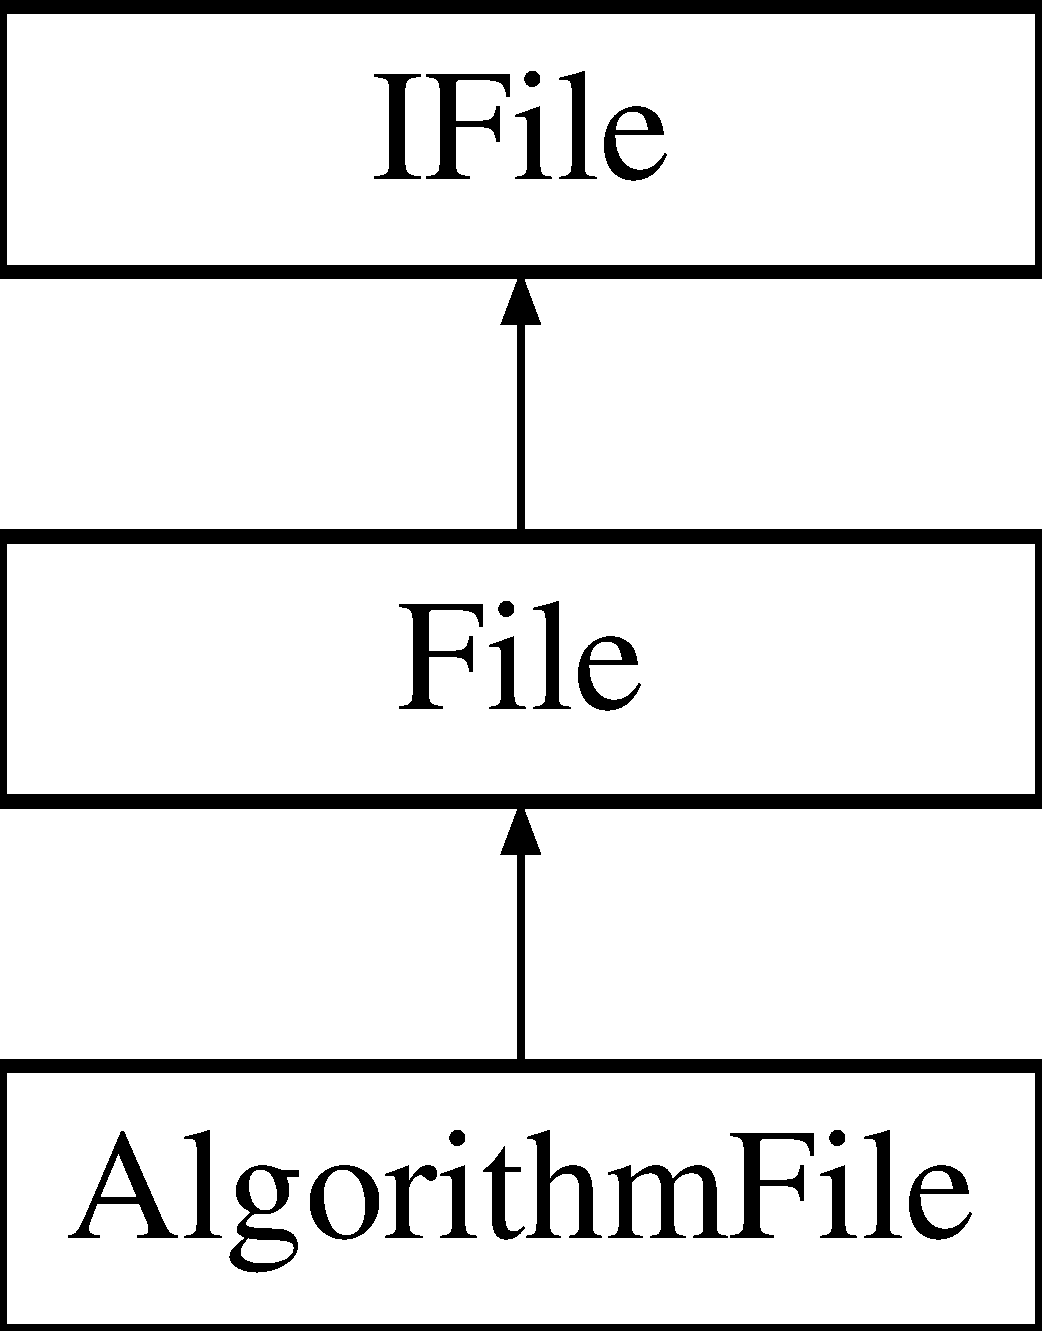
\includegraphics[height=3.000000cm]{class_algorithm_file}
\end{center}
\end{figure}
\subsection*{Metody publiczne}
\begin{DoxyCompactItemize}
\item 
Q\+String\+List \hyperlink{class_algorithm_file_aad65cdb6b287b17fed79d2419a0a38de}{prepare\+Content\+To\+Set} ()
\begin{DoxyCompactList}\small\item\em prepare\+Content\+To\+Set -\/ metoda przygotowuje zawartość pliku dla pola skrypt obiektu klasy \hyperlink{class_algorithm}{Algorithm} \end{DoxyCompactList}\item 
Q\+String \hyperlink{class_algorithm_file_ad61d9a5c9f537b8c0c985fb0810fc6fb}{prepare\+Content\+To\+Save} (\hyperlink{class_data_manager}{Data\+Manager} \&\+\_\+data\+Manager, char c)
\begin{DoxyCompactList}\small\item\em prepare\+Content\+To\+Save -\/ metoda przygotowuje skrypt do zapisu w pliu \end{DoxyCompactList}\end{DoxyCompactItemize}
\subsection*{Dodatkowe Dziedziczone Składowe}


\subsection{Opis szczegółowy}
Klasa \hyperlink{class_algorithm_file}{Algorithm\+File} -\/ obiekty tej klasy przechowują informacje o pliku z którego jest wczytywany algorytm. 

\subsection{Dokumentacja funkcji składowych}
\hypertarget{class_algorithm_file_ad61d9a5c9f537b8c0c985fb0810fc6fb}{\index{Algorithm\+File@{Algorithm\+File}!prepare\+Content\+To\+Save@{prepare\+Content\+To\+Save}}
\index{prepare\+Content\+To\+Save@{prepare\+Content\+To\+Save}!Algorithm\+File@{Algorithm\+File}}
\subsubsection[{prepare\+Content\+To\+Save}]{\setlength{\rightskip}{0pt plus 5cm}Q\+String Algorithm\+File\+::prepare\+Content\+To\+Save (
\begin{DoxyParamCaption}
\item[{{\bf Data\+Manager} \&}]{\+\_\+data\+Manager, }
\item[{char}]{c}
\end{DoxyParamCaption}
)\hspace{0.3cm}{\ttfamily [virtual]}}}\label{class_algorithm_file_ad61d9a5c9f537b8c0c985fb0810fc6fb}


prepare\+Content\+To\+Save -\/ metoda przygotowuje skrypt do zapisu w pliu 


\begin{DoxyParams}{Parametry}
{\em \+\_\+data\+Manager} & -\/ parametr niezbędny do pobrania informacji o aktualnie wybranym algorytmie \\
\hline
{\em c} & -\/ parametr informujący o tym co będzie zapisane \\
\hline
\end{DoxyParams}
\begin{DoxyReturn}{Zwraca}
-\/ przygotowana treść do zapisu 
\end{DoxyReturn}


Implementuje \hyperlink{class_file}{File}.

\hypertarget{class_algorithm_file_aad65cdb6b287b17fed79d2419a0a38de}{\index{Algorithm\+File@{Algorithm\+File}!prepare\+Content\+To\+Set@{prepare\+Content\+To\+Set}}
\index{prepare\+Content\+To\+Set@{prepare\+Content\+To\+Set}!Algorithm\+File@{Algorithm\+File}}
\subsubsection[{prepare\+Content\+To\+Set}]{\setlength{\rightskip}{0pt plus 5cm}Q\+String\+List Algorithm\+File\+::prepare\+Content\+To\+Set (
\begin{DoxyParamCaption}
{}
\end{DoxyParamCaption}
)\hspace{0.3cm}{\ttfamily [virtual]}}}\label{class_algorithm_file_aad65cdb6b287b17fed79d2419a0a38de}


prepare\+Content\+To\+Set -\/ metoda przygotowuje zawartość pliku dla pola skrypt obiektu klasy \hyperlink{class_algorithm}{Algorithm} 

\begin{DoxyReturn}{Zwraca}
-\/ przygotowana treść do ustawienia w obiecie klasy \hyperlink{class_algorithm}{Algorithm} 
\end{DoxyReturn}


Implementuje \hyperlink{class_file}{File}.



Dokumentacja dla tej klasy została wygenerowana z plików\+:\begin{DoxyCompactItemize}
\item 
C\+:/\+Users/\+Marcin/\+Desktop/\+Snakes\+\_\+snakes/algorithmfile.\+h\item 
C\+:/\+Users/\+Marcin/\+Desktop/\+Snakes\+\_\+snakes/algorithmfile.\+cpp\end{DoxyCompactItemize}

\hypertarget{class_data_manager}{\section{Dokumentacja klasy Data\+Manager}
\label{class_data_manager}\index{Data\+Manager@{Data\+Manager}}
}


Klasa \hyperlink{class_data_manager}{Data\+Manager} -\/ obiekt tej klasy zarządza przetwarzanymi w programie danymi, tj. algorytmami i seriami.  




{\ttfamily \#include $<$datamanager.\+h$>$}

\subsection*{Metody publiczne}
\begin{DoxyCompactItemize}
\item 
\hyperlink{class_algorithm}{Algorithm} $\ast$ \hyperlink{class_data_manager_a8d0afcc6bd82efea1a087a77ba046df0}{get\+Current\+Algorithm} ()
\begin{DoxyCompactList}\small\item\em get\+Current\+Algorithm -\/ metoda pobiera wskaźnik na aktualnie wybrany algorytm \end{DoxyCompactList}\item 
std\+::vector$<$ \hyperlink{class_algorithm}{Algorithm} $\ast$ $>$ \hyperlink{class_data_manager_afb85e233fe55a742241597aeb988c6ae}{get\+Algorithms} ()
\begin{DoxyCompactList}\small\item\em get\+Algorithms -\/ metoda pobiera wskaźniki na wszystkie algorytmy \end{DoxyCompactList}\item 
void \hyperlink{class_data_manager_ac840fe3df9dcb8c7fed38c40d817fbc4}{set\+Current\+Algorithm} (int \+\_\+algorithm\+Row)
\begin{DoxyCompactList}\small\item\em set\+Current\+Algorithm -\/ metoda ustawia wskaźnik na aktualnie wybrany algorytm \end{DoxyCompactList}\item 
\hyperlink{class_series}{Series} $\ast$ \hyperlink{class_data_manager_a7071330f82722bfa47994c90325c76ec}{get\+Current\+Input\+Series} ()
\begin{DoxyCompactList}\small\item\em get\+Current\+Input\+Series -\/ metoda pobiera wskaźnik na aktualnie wybraną serię wejściową \end{DoxyCompactList}\item 
std\+::vector$<$ \hyperlink{class_series}{Series} $\ast$ $>$ \hyperlink{class_data_manager_afb4de666c7412d0d1892e7e54ed82aaf}{get\+Input\+Series} ()
\begin{DoxyCompactList}\small\item\em get\+Input\+Series -\/ metoda pobiera wskaźniki na wszystkie serie wejściowe \end{DoxyCompactList}\item 
void \hyperlink{class_data_manager_a2c9efa56273db676e98641c1d84bbee2}{set\+Current\+Input\+Series} (int \+\_\+input\+Series\+Row)
\begin{DoxyCompactList}\small\item\em set\+Current\+Input\+Series -\/ metoda ustawia wskaźnik na aktualnie wybraną serię wejściową \end{DoxyCompactList}\item 
\hyperlink{class_series}{Series} $\ast$ \hyperlink{class_data_manager_a86ad97b64097b93db9f8cd02a73c801c}{get\+Current\+Output\+Series} ()
\begin{DoxyCompactList}\small\item\em get\+Current\+Output\+Series -\/ metoda pobiera wskaźnik na aktualnie wybraną serię wyjściową \end{DoxyCompactList}\item 
std\+::vector$<$ \hyperlink{class_series}{Series} $\ast$ $>$ \hyperlink{class_data_manager_a36454e708a2041da015549ea38877a16}{get\+Output\+Series} ()
\begin{DoxyCompactList}\small\item\em get\+Output\+Series -\/ metoda pobiera wskaźniki na wszystkie serie wyjściowe \end{DoxyCompactList}\item 
void \hyperlink{class_data_manager_a18a047d7c27dac16ad97e0ab08ab1a11}{set\+Current\+Output\+Series} (int \+\_\+output\+Series)
\begin{DoxyCompactList}\small\item\em set\+Current\+Output\+Series -\/ metoda ustawia wskaźnik na aktualnie wybraną serię wyjściową \end{DoxyCompactList}\item 
void \hyperlink{class_data_manager_ac7adc63ceee86ef18b88408d536468fd}{add\+Series\+From\+File} (\hyperlink{class_i_file}{I\+File} $\ast$\+\_\+file)
\begin{DoxyCompactList}\small\item\em add\+Series\+From\+File -\/ metoda dodaje serię z pliku \end{DoxyCompactList}\item 
void \hyperlink{class_data_manager_ab3095e58be93fcb77a4f4814f08fb3ec}{delete\+Series} (int \+\_\+current\+Series, char \+\_\+which\+Series)
\begin{DoxyCompactList}\small\item\em delete\+Series -\/ metoda usuwa serię \end{DoxyCompactList}\item 
void \hyperlink{class_data_manager_a1c252d92169045d9ac646dc264de9397}{add\+New\+Algorithm} (Q\+String \+\_\+name)
\begin{DoxyCompactList}\small\item\em add\+New\+Algorithm -\/ metoda dodaje nowy algorytm \end{DoxyCompactList}\item 
void \hyperlink{class_data_manager_a2664e4d4e1026d9eccde04def2fa0278}{add\+Algorithm\+From\+File} (\hyperlink{class_i_file}{I\+File} $\ast$\+\_\+file)
\begin{DoxyCompactList}\small\item\em add\+Algorithm\+From\+File -\/ metoda dodaje algorytm z pliku \end{DoxyCompactList}\item 
void \hyperlink{class_data_manager_a98d1a9bb8759afe78b86a1a9c5c891fd}{delete\+Algorithm} (int \+\_\+current\+Algorithm)
\begin{DoxyCompactList}\small\item\em delete\+Algorithm -\/ metoda usuwa algorytm \end{DoxyCompactList}\item 
void \hyperlink{class_data_manager_afad3b8ee5ba4463d53da7406bec8e2aa}{prepare\+New\+Series} (Q\+String \+\_\+name)
\begin{DoxyCompactList}\small\item\em prepare\+New\+Series -\/ metoda przygotowuje nową serię wyjściową \end{DoxyCompactList}\end{DoxyCompactItemize}


\subsection{Opis szczegółowy}
Klasa \hyperlink{class_data_manager}{Data\+Manager} -\/ obiekt tej klasy zarządza przetwarzanymi w programie danymi, tj. algorytmami i seriami. 

\subsection{Dokumentacja funkcji składowych}
\hypertarget{class_data_manager_a2664e4d4e1026d9eccde04def2fa0278}{\index{Data\+Manager@{Data\+Manager}!add\+Algorithm\+From\+File@{add\+Algorithm\+From\+File}}
\index{add\+Algorithm\+From\+File@{add\+Algorithm\+From\+File}!Data\+Manager@{Data\+Manager}}
\subsubsection[{add\+Algorithm\+From\+File}]{\setlength{\rightskip}{0pt plus 5cm}void Data\+Manager\+::add\+Algorithm\+From\+File (
\begin{DoxyParamCaption}
\item[{{\bf I\+File} $\ast$}]{\+\_\+file}
\end{DoxyParamCaption}
)}}\label{class_data_manager_a2664e4d4e1026d9eccde04def2fa0278}


add\+Algorithm\+From\+File -\/ metoda dodaje algorytm z pliku 


\begin{DoxyParams}{Parametry}
{\em \+\_\+file} & -\/ obsługiwany plik \\
\hline
\end{DoxyParams}
\hypertarget{class_data_manager_a1c252d92169045d9ac646dc264de9397}{\index{Data\+Manager@{Data\+Manager}!add\+New\+Algorithm@{add\+New\+Algorithm}}
\index{add\+New\+Algorithm@{add\+New\+Algorithm}!Data\+Manager@{Data\+Manager}}
\subsubsection[{add\+New\+Algorithm}]{\setlength{\rightskip}{0pt plus 5cm}void Data\+Manager\+::add\+New\+Algorithm (
\begin{DoxyParamCaption}
\item[{Q\+String}]{\+\_\+name}
\end{DoxyParamCaption}
)}}\label{class_data_manager_a1c252d92169045d9ac646dc264de9397}


add\+New\+Algorithm -\/ metoda dodaje nowy algorytm 


\begin{DoxyParams}{Parametry}
{\em \+\_\+name} & -\/ nazwa nowego algorytmu \\
\hline
\end{DoxyParams}
\hypertarget{class_data_manager_ac7adc63ceee86ef18b88408d536468fd}{\index{Data\+Manager@{Data\+Manager}!add\+Series\+From\+File@{add\+Series\+From\+File}}
\index{add\+Series\+From\+File@{add\+Series\+From\+File}!Data\+Manager@{Data\+Manager}}
\subsubsection[{add\+Series\+From\+File}]{\setlength{\rightskip}{0pt plus 5cm}void Data\+Manager\+::add\+Series\+From\+File (
\begin{DoxyParamCaption}
\item[{{\bf I\+File} $\ast$}]{\+\_\+file}
\end{DoxyParamCaption}
)}}\label{class_data_manager_ac7adc63ceee86ef18b88408d536468fd}


add\+Series\+From\+File -\/ metoda dodaje serię z pliku 


\begin{DoxyParams}{Parametry}
{\em \+\_\+file} & -\/ obsługiwany plik \\
\hline
\end{DoxyParams}
\hypertarget{class_data_manager_a98d1a9bb8759afe78b86a1a9c5c891fd}{\index{Data\+Manager@{Data\+Manager}!delete\+Algorithm@{delete\+Algorithm}}
\index{delete\+Algorithm@{delete\+Algorithm}!Data\+Manager@{Data\+Manager}}
\subsubsection[{delete\+Algorithm}]{\setlength{\rightskip}{0pt plus 5cm}void Data\+Manager\+::delete\+Algorithm (
\begin{DoxyParamCaption}
\item[{int}]{\+\_\+current\+Algorithm}
\end{DoxyParamCaption}
)}}\label{class_data_manager_a98d1a9bb8759afe78b86a1a9c5c891fd}


delete\+Algorithm -\/ metoda usuwa algorytm 


\begin{DoxyParams}{Parametry}
{\em \+\_\+current\+Algorithm} & -\/ numer wiersza wybranego aktualnie algorytmu w okienku głównym \\
\hline
\end{DoxyParams}
\hypertarget{class_data_manager_ab3095e58be93fcb77a4f4814f08fb3ec}{\index{Data\+Manager@{Data\+Manager}!delete\+Series@{delete\+Series}}
\index{delete\+Series@{delete\+Series}!Data\+Manager@{Data\+Manager}}
\subsubsection[{delete\+Series}]{\setlength{\rightskip}{0pt plus 5cm}void Data\+Manager\+::delete\+Series (
\begin{DoxyParamCaption}
\item[{int}]{\+\_\+current\+Series, }
\item[{char}]{\+\_\+which\+Series}
\end{DoxyParamCaption}
)}}\label{class_data_manager_ab3095e58be93fcb77a4f4814f08fb3ec}


delete\+Series -\/ metoda usuwa serię 


\begin{DoxyParams}{Parametry}
{\em \+\_\+current\+Series} & -\/ numer wiersza wybranej aktualnie serii wejściowej/wyjściowej w okienku głównym \\
\hline
{\em \+\_\+which\+Series} & -\/ parametr informujący o tym która seria jest do usunięcia\+: wejściowa czy wyjściowa \\
\hline
\end{DoxyParams}
\hypertarget{class_data_manager_afb85e233fe55a742241597aeb988c6ae}{\index{Data\+Manager@{Data\+Manager}!get\+Algorithms@{get\+Algorithms}}
\index{get\+Algorithms@{get\+Algorithms}!Data\+Manager@{Data\+Manager}}
\subsubsection[{get\+Algorithms}]{\setlength{\rightskip}{0pt plus 5cm}std\+::vector$<$ {\bf Algorithm} $\ast$ $>$ Data\+Manager\+::get\+Algorithms (
\begin{DoxyParamCaption}
{}
\end{DoxyParamCaption}
)}}\label{class_data_manager_afb85e233fe55a742241597aeb988c6ae}


get\+Algorithms -\/ metoda pobiera wskaźniki na wszystkie algorytmy 

\begin{DoxyReturn}{Zwraca}
-\/ wektor wskaźników na algorytmy 
\end{DoxyReturn}
\hypertarget{class_data_manager_a8d0afcc6bd82efea1a087a77ba046df0}{\index{Data\+Manager@{Data\+Manager}!get\+Current\+Algorithm@{get\+Current\+Algorithm}}
\index{get\+Current\+Algorithm@{get\+Current\+Algorithm}!Data\+Manager@{Data\+Manager}}
\subsubsection[{get\+Current\+Algorithm}]{\setlength{\rightskip}{0pt plus 5cm}{\bf Algorithm} $\ast$ Data\+Manager\+::get\+Current\+Algorithm (
\begin{DoxyParamCaption}
{}
\end{DoxyParamCaption}
)}}\label{class_data_manager_a8d0afcc6bd82efea1a087a77ba046df0}


get\+Current\+Algorithm -\/ metoda pobiera wskaźnik na aktualnie wybrany algorytm 

\begin{DoxyReturn}{Zwraca}
-\/ wskaźnik do aktualnie wybranego algorytmu 
\end{DoxyReturn}
\hypertarget{class_data_manager_a7071330f82722bfa47994c90325c76ec}{\index{Data\+Manager@{Data\+Manager}!get\+Current\+Input\+Series@{get\+Current\+Input\+Series}}
\index{get\+Current\+Input\+Series@{get\+Current\+Input\+Series}!Data\+Manager@{Data\+Manager}}
\subsubsection[{get\+Current\+Input\+Series}]{\setlength{\rightskip}{0pt plus 5cm}{\bf Series} $\ast$ Data\+Manager\+::get\+Current\+Input\+Series (
\begin{DoxyParamCaption}
{}
\end{DoxyParamCaption}
)}}\label{class_data_manager_a7071330f82722bfa47994c90325c76ec}


get\+Current\+Input\+Series -\/ metoda pobiera wskaźnik na aktualnie wybraną serię wejściową 

\begin{DoxyReturn}{Zwraca}
-\/ wskaźni do aktualnie wybranej serii wejściowej 
\end{DoxyReturn}
\hypertarget{class_data_manager_a86ad97b64097b93db9f8cd02a73c801c}{\index{Data\+Manager@{Data\+Manager}!get\+Current\+Output\+Series@{get\+Current\+Output\+Series}}
\index{get\+Current\+Output\+Series@{get\+Current\+Output\+Series}!Data\+Manager@{Data\+Manager}}
\subsubsection[{get\+Current\+Output\+Series}]{\setlength{\rightskip}{0pt plus 5cm}{\bf Series} $\ast$ Data\+Manager\+::get\+Current\+Output\+Series (
\begin{DoxyParamCaption}
{}
\end{DoxyParamCaption}
)}}\label{class_data_manager_a86ad97b64097b93db9f8cd02a73c801c}


get\+Current\+Output\+Series -\/ metoda pobiera wskaźnik na aktualnie wybraną serię wyjściową 

\begin{DoxyReturn}{Zwraca}
-\/ wskaźnik do aktualnie wybranej serii wyjściowej 
\end{DoxyReturn}
\hypertarget{class_data_manager_afb4de666c7412d0d1892e7e54ed82aaf}{\index{Data\+Manager@{Data\+Manager}!get\+Input\+Series@{get\+Input\+Series}}
\index{get\+Input\+Series@{get\+Input\+Series}!Data\+Manager@{Data\+Manager}}
\subsubsection[{get\+Input\+Series}]{\setlength{\rightskip}{0pt plus 5cm}std\+::vector$<$ {\bf Series} $\ast$ $>$ Data\+Manager\+::get\+Input\+Series (
\begin{DoxyParamCaption}
{}
\end{DoxyParamCaption}
)}}\label{class_data_manager_afb4de666c7412d0d1892e7e54ed82aaf}


get\+Input\+Series -\/ metoda pobiera wskaźniki na wszystkie serie wejściowe 

\begin{DoxyReturn}{Zwraca}
-\/ wektor wskaźników na serie wejściowe 
\end{DoxyReturn}
\hypertarget{class_data_manager_a36454e708a2041da015549ea38877a16}{\index{Data\+Manager@{Data\+Manager}!get\+Output\+Series@{get\+Output\+Series}}
\index{get\+Output\+Series@{get\+Output\+Series}!Data\+Manager@{Data\+Manager}}
\subsubsection[{get\+Output\+Series}]{\setlength{\rightskip}{0pt plus 5cm}std\+::vector$<$ {\bf Series} $\ast$ $>$ Data\+Manager\+::get\+Output\+Series (
\begin{DoxyParamCaption}
{}
\end{DoxyParamCaption}
)}}\label{class_data_manager_a36454e708a2041da015549ea38877a16}


get\+Output\+Series -\/ metoda pobiera wskaźniki na wszystkie serie wyjściowe 

\begin{DoxyReturn}{Zwraca}
-\/ wektor wskaźników na serie wyjściowe 
\end{DoxyReturn}
\hypertarget{class_data_manager_afad3b8ee5ba4463d53da7406bec8e2aa}{\index{Data\+Manager@{Data\+Manager}!prepare\+New\+Series@{prepare\+New\+Series}}
\index{prepare\+New\+Series@{prepare\+New\+Series}!Data\+Manager@{Data\+Manager}}
\subsubsection[{prepare\+New\+Series}]{\setlength{\rightskip}{0pt plus 5cm}void Data\+Manager\+::prepare\+New\+Series (
\begin{DoxyParamCaption}
\item[{Q\+String}]{\+\_\+name}
\end{DoxyParamCaption}
)}}\label{class_data_manager_afad3b8ee5ba4463d53da7406bec8e2aa}


prepare\+New\+Series -\/ metoda przygotowuje nową serię wyjściową 


\begin{DoxyParams}{Parametry}
{\em \+\_\+name} & -\/ nazwa nowej serii \\
\hline
\end{DoxyParams}
\hypertarget{class_data_manager_ac840fe3df9dcb8c7fed38c40d817fbc4}{\index{Data\+Manager@{Data\+Manager}!set\+Current\+Algorithm@{set\+Current\+Algorithm}}
\index{set\+Current\+Algorithm@{set\+Current\+Algorithm}!Data\+Manager@{Data\+Manager}}
\subsubsection[{set\+Current\+Algorithm}]{\setlength{\rightskip}{0pt plus 5cm}void Data\+Manager\+::set\+Current\+Algorithm (
\begin{DoxyParamCaption}
\item[{int}]{\+\_\+algorithm\+Row}
\end{DoxyParamCaption}
)}}\label{class_data_manager_ac840fe3df9dcb8c7fed38c40d817fbc4}


set\+Current\+Algorithm -\/ metoda ustawia wskaźnik na aktualnie wybrany algorytm 


\begin{DoxyParams}{Parametry}
{\em \+\_\+algorithm\+Row} & -\/ numer wiersza wybranego algorytmu w okienku głównym \\
\hline
\end{DoxyParams}
\hypertarget{class_data_manager_a2c9efa56273db676e98641c1d84bbee2}{\index{Data\+Manager@{Data\+Manager}!set\+Current\+Input\+Series@{set\+Current\+Input\+Series}}
\index{set\+Current\+Input\+Series@{set\+Current\+Input\+Series}!Data\+Manager@{Data\+Manager}}
\subsubsection[{set\+Current\+Input\+Series}]{\setlength{\rightskip}{0pt plus 5cm}void Data\+Manager\+::set\+Current\+Input\+Series (
\begin{DoxyParamCaption}
\item[{int}]{\+\_\+input\+Series\+Row}
\end{DoxyParamCaption}
)}}\label{class_data_manager_a2c9efa56273db676e98641c1d84bbee2}


set\+Current\+Input\+Series -\/ metoda ustawia wskaźnik na aktualnie wybraną serię wejściową 


\begin{DoxyParams}{Parametry}
{\em \+\_\+input\+Series\+Row} & -\/ numer wiersza wybranej serii wejściowej w okienku głównym \\
\hline
\end{DoxyParams}
\hypertarget{class_data_manager_a18a047d7c27dac16ad97e0ab08ab1a11}{\index{Data\+Manager@{Data\+Manager}!set\+Current\+Output\+Series@{set\+Current\+Output\+Series}}
\index{set\+Current\+Output\+Series@{set\+Current\+Output\+Series}!Data\+Manager@{Data\+Manager}}
\subsubsection[{set\+Current\+Output\+Series}]{\setlength{\rightskip}{0pt plus 5cm}void Data\+Manager\+::set\+Current\+Output\+Series (
\begin{DoxyParamCaption}
\item[{int}]{\+\_\+output\+Series}
\end{DoxyParamCaption}
)}}\label{class_data_manager_a18a047d7c27dac16ad97e0ab08ab1a11}


set\+Current\+Output\+Series -\/ metoda ustawia wskaźnik na aktualnie wybraną serię wyjściową 


\begin{DoxyParams}{Parametry}
{\em \+\_\+output\+Series} & -\/ numer wiersza wybranej serii wyjściowej w okienku głównym \\
\hline
\end{DoxyParams}


Dokumentacja dla tej klasy została wygenerowana z plików\+:\begin{DoxyCompactItemize}
\item 
C\+:/\+Users/\+Marcin/\+Desktop/\+Snakes\+\_\+snakes/datamanager.\+h\item 
C\+:/\+Users/\+Marcin/\+Desktop/\+Snakes\+\_\+snakes/datamanager.\+cpp\end{DoxyCompactItemize}

\hypertarget{class_file}{\section{Dokumentacja klasy File}
\label{class_file}\index{File@{File}}
}


Klasa \hyperlink{class_file}{File} -\/ obiekty tej klasy przechowują informacje o pliku z którego są wczytywane dane.  




{\ttfamily \#include $<$file.\+h$>$}

Diagram dziedziczenia dla File\begin{figure}[H]
\begin{center}
\leavevmode
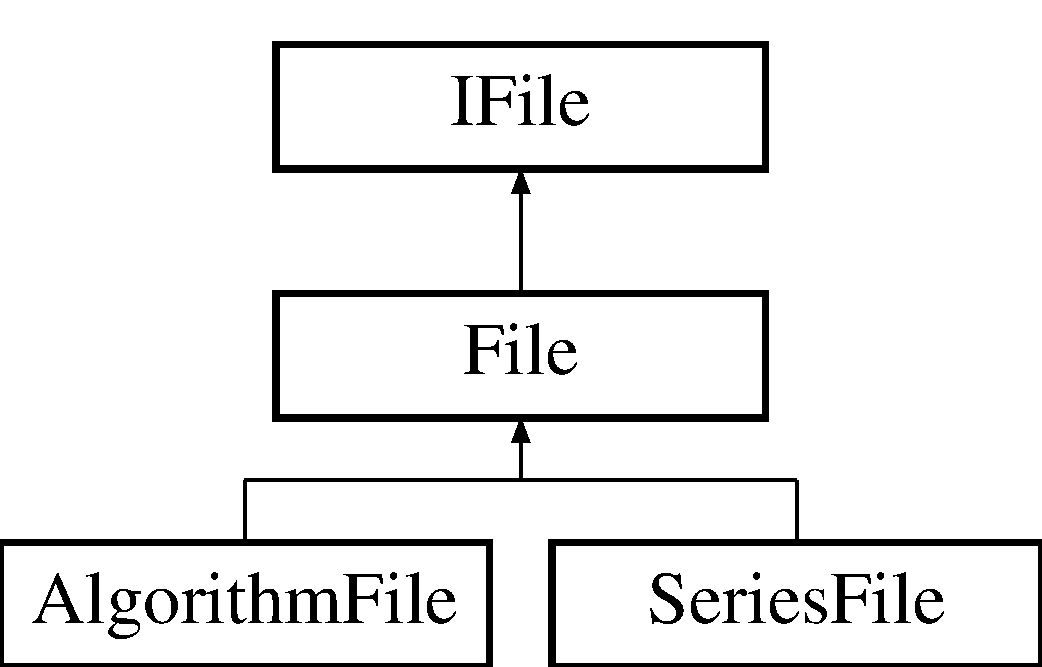
\includegraphics[height=3.000000cm]{class_file}
\end{center}
\end{figure}
\subsection*{Metody publiczne}
\begin{DoxyCompactItemize}
\item 
Q\+String \hyperlink{class_file_a55683b67c0f7f53d4f2ee544587a1478}{get\+Name} ()
\begin{DoxyCompactList}\small\item\em get\+Name -\/ metoda pobiera nazwę pliku \end{DoxyCompactList}\item 
void \hyperlink{class_file_a1a2f0af57b4cb416d07b4c7f4a1ef04a}{set\+Name} (Q\+String \+\_\+name)
\begin{DoxyCompactList}\small\item\em set\+Name -\/ metoda ustawia nazwę pliku \end{DoxyCompactList}\item 
Q\+String \hyperlink{class_file_a1fdbcf449f0e8365b3d5cf003909b1b5}{get\+File\+Path} ()
\begin{DoxyCompactList}\small\item\em get\+File\+Path -\/ metoda pobiera ścieżkę do pliku \end{DoxyCompactList}\item 
void \hyperlink{class_file_ad7216b449a5868da61388cde79070d6f}{set\+File\+Path} (Q\+String \+\_\+path)
\begin{DoxyCompactList}\small\item\em set\+File\+Path -\/ metoda ustawia ścieżkę do pliku \end{DoxyCompactList}\item 
Q\+String \hyperlink{class_file_ac80dd9634f10f53494c4fd5265483c21}{get\+Content} ()
\begin{DoxyCompactList}\small\item\em get\+Content -\/ metoda pobiera zawartość pliku \end{DoxyCompactList}\item 
void \hyperlink{class_file_a38cb05c7dde38d6bd8abb62e85e42404}{set\+Content} (Q\+String \+\_\+content)
\begin{DoxyCompactList}\small\item\em set\+Content -\/ metoda ustawia zawartość pliku \end{DoxyCompactList}\end{DoxyCompactItemize}
\subsection*{Atrybuty chronione}
\begin{DoxyCompactItemize}
\item 
\hypertarget{class_file_ad5ee1de5d6d6c5b792f3b357993f08fc}{Q\+String \hyperlink{class_file_ad5ee1de5d6d6c5b792f3b357993f08fc}{file\+Name}}\label{class_file_ad5ee1de5d6d6c5b792f3b357993f08fc}

\begin{DoxyCompactList}\small\item\em file\+Name -\/ nazwa pliku \end{DoxyCompactList}\item 
\hypertarget{class_file_a2f4b24c592c50ad086bc0e6f1a3b5b41}{Q\+String \hyperlink{class_file_a2f4b24c592c50ad086bc0e6f1a3b5b41}{file\+Path}}\label{class_file_a2f4b24c592c50ad086bc0e6f1a3b5b41}

\begin{DoxyCompactList}\small\item\em file\+Path -\/ ścieżka do pliku \end{DoxyCompactList}\item 
\hypertarget{class_file_a95208d4aefbc2f99f5c9405468409c4a}{Q\+String \hyperlink{class_file_a95208d4aefbc2f99f5c9405468409c4a}{file\+Content}}\label{class_file_a95208d4aefbc2f99f5c9405468409c4a}

\begin{DoxyCompactList}\small\item\em file\+Content -\/ zwartość pliku \end{DoxyCompactList}\end{DoxyCompactItemize}


\subsection{Opis szczegółowy}
Klasa \hyperlink{class_file}{File} -\/ obiekty tej klasy przechowują informacje o pliku z którego są wczytywane dane. 

\subsection{Dokumentacja funkcji składowych}
\hypertarget{class_file_ac80dd9634f10f53494c4fd5265483c21}{\index{File@{File}!get\+Content@{get\+Content}}
\index{get\+Content@{get\+Content}!File@{File}}
\subsubsection[{get\+Content}]{\setlength{\rightskip}{0pt plus 5cm}Q\+String File\+::get\+Content (
\begin{DoxyParamCaption}
{}
\end{DoxyParamCaption}
)}}\label{class_file_ac80dd9634f10f53494c4fd5265483c21}


get\+Content -\/ metoda pobiera zawartość pliku 

\begin{DoxyReturn}{Zwraca}
-\/ zawartość pliku 
\end{DoxyReturn}
\hypertarget{class_file_a1fdbcf449f0e8365b3d5cf003909b1b5}{\index{File@{File}!get\+File\+Path@{get\+File\+Path}}
\index{get\+File\+Path@{get\+File\+Path}!File@{File}}
\subsubsection[{get\+File\+Path}]{\setlength{\rightskip}{0pt plus 5cm}Q\+String File\+::get\+File\+Path (
\begin{DoxyParamCaption}
{}
\end{DoxyParamCaption}
)}}\label{class_file_a1fdbcf449f0e8365b3d5cf003909b1b5}


get\+File\+Path -\/ metoda pobiera ścieżkę do pliku 

\begin{DoxyReturn}{Zwraca}
-\/ ścieżka do pliku 
\end{DoxyReturn}
\hypertarget{class_file_a55683b67c0f7f53d4f2ee544587a1478}{\index{File@{File}!get\+Name@{get\+Name}}
\index{get\+Name@{get\+Name}!File@{File}}
\subsubsection[{get\+Name}]{\setlength{\rightskip}{0pt plus 5cm}Q\+String File\+::get\+Name (
\begin{DoxyParamCaption}
{}
\end{DoxyParamCaption}
)\hspace{0.3cm}{\ttfamily [virtual]}}}\label{class_file_a55683b67c0f7f53d4f2ee544587a1478}


get\+Name -\/ metoda pobiera nazwę pliku 

\begin{DoxyReturn}{Zwraca}
-\/ nazwa pliku 
\end{DoxyReturn}


Implementuje \hyperlink{class_i_file}{I\+File}.

\hypertarget{class_file_a38cb05c7dde38d6bd8abb62e85e42404}{\index{File@{File}!set\+Content@{set\+Content}}
\index{set\+Content@{set\+Content}!File@{File}}
\subsubsection[{set\+Content}]{\setlength{\rightskip}{0pt plus 5cm}void File\+::set\+Content (
\begin{DoxyParamCaption}
\item[{Q\+String}]{\+\_\+content}
\end{DoxyParamCaption}
)}}\label{class_file_a38cb05c7dde38d6bd8abb62e85e42404}


set\+Content -\/ metoda ustawia zawartość pliku 


\begin{DoxyParams}{Parametry}
{\em \+\_\+content} & -\/ zawartość pliku do ustawienia \\
\hline
\end{DoxyParams}
\hypertarget{class_file_ad7216b449a5868da61388cde79070d6f}{\index{File@{File}!set\+File\+Path@{set\+File\+Path}}
\index{set\+File\+Path@{set\+File\+Path}!File@{File}}
\subsubsection[{set\+File\+Path}]{\setlength{\rightskip}{0pt plus 5cm}void File\+::set\+File\+Path (
\begin{DoxyParamCaption}
\item[{Q\+String}]{\+\_\+path}
\end{DoxyParamCaption}
)}}\label{class_file_ad7216b449a5868da61388cde79070d6f}


set\+File\+Path -\/ metoda ustawia ścieżkę do pliku 


\begin{DoxyParams}{Parametry}
{\em \+\_\+path} & -\/ ścieżka do pliku do ustawienia \\
\hline
\end{DoxyParams}
\hypertarget{class_file_a1a2f0af57b4cb416d07b4c7f4a1ef04a}{\index{File@{File}!set\+Name@{set\+Name}}
\index{set\+Name@{set\+Name}!File@{File}}
\subsubsection[{set\+Name}]{\setlength{\rightskip}{0pt plus 5cm}void File\+::set\+Name (
\begin{DoxyParamCaption}
\item[{Q\+String}]{\+\_\+name}
\end{DoxyParamCaption}
)}}\label{class_file_a1a2f0af57b4cb416d07b4c7f4a1ef04a}


set\+Name -\/ metoda ustawia nazwę pliku 


\begin{DoxyParams}{Parametry}
{\em \+\_\+name} & -\/ nazwa pliku do ustawienia \\
\hline
\end{DoxyParams}


Dokumentacja dla tej klasy została wygenerowana z plików\+:\begin{DoxyCompactItemize}
\item 
C\+:/\+Users/\+Marcin/\+Desktop/\+Snakes\+\_\+snakes/file.\+h\item 
C\+:/\+Users/\+Marcin/\+Desktop/\+Snakes\+\_\+snakes/file.\+cpp\end{DoxyCompactItemize}

\hypertarget{class_file_manager}{\section{Dokumentacja klasy File\+Manager}
\label{class_file_manager}\index{File\+Manager@{File\+Manager}}
}


Klasa \hyperlink{class_file_manager}{File\+Manager} -\/ obiekt tej klasy służy do obsługi plików wczytywanych do programu.  




{\ttfamily \#include $<$filemanager.\+h$>$}

\subsection*{Metody publiczne}
\begin{DoxyCompactItemize}
\item 
\hyperlink{class_file}{File} $\ast$ \hyperlink{class_file_manager_aa7e765d8eab798ee2adef644e163a84a}{get\+File} ()
\begin{DoxyCompactList}\small\item\em get\+File -\/ metoda pobiera wskaźnik na aktualnie obsługiwanego pliku \end{DoxyCompactList}\item 
void \hyperlink{class_file_manager_a9d03f4076a7f1d933d47809d039a6377}{set\+File} (\hyperlink{class_file}{File} $\ast$\+\_\+file)
\begin{DoxyCompactList}\small\item\em set\+File -\/ metoda ustawia wskaźnik na aktualnie obsługiwany plik \end{DoxyCompactList}\item 
bool \hyperlink{class_file_manager_a84ffd312c627e3e28501fd3169b3d59d}{open\+File} (char \+\_\+what\+To\+Load, Q\+String \+\_\+path)
\begin{DoxyCompactList}\small\item\em open\+File -\/ metoda służy do otwierania pliku \end{DoxyCompactList}\item 
bool \hyperlink{class_file_manager_a7718e386811bca53267f3cfc09a15906}{save\+File} (char \+\_\+what\+To\+Save, Q\+String \+\_\+path, \hyperlink{class_data_manager}{Data\+Manager} \&\+\_\+data\+Manager)
\begin{DoxyCompactList}\small\item\em save\+File -\/ metoda służy do zapisywania pliku \end{DoxyCompactList}\end{DoxyCompactItemize}


\subsection{Opis szczegółowy}
Klasa \hyperlink{class_file_manager}{File\+Manager} -\/ obiekt tej klasy służy do obsługi plików wczytywanych do programu. 

\subsection{Dokumentacja funkcji składowych}
\hypertarget{class_file_manager_aa7e765d8eab798ee2adef644e163a84a}{\index{File\+Manager@{File\+Manager}!get\+File@{get\+File}}
\index{get\+File@{get\+File}!File\+Manager@{File\+Manager}}
\subsubsection[{get\+File}]{\setlength{\rightskip}{0pt plus 5cm}{\bf File} $\ast$ File\+Manager\+::get\+File (
\begin{DoxyParamCaption}
{}
\end{DoxyParamCaption}
)}}\label{class_file_manager_aa7e765d8eab798ee2adef644e163a84a}


get\+File -\/ metoda pobiera wskaźnik na aktualnie obsługiwanego pliku 

\begin{DoxyReturn}{Zwraca}
-\/ wskaźni do aktualnie obsługiwanego pliku 
\end{DoxyReturn}
\hypertarget{class_file_manager_a84ffd312c627e3e28501fd3169b3d59d}{\index{File\+Manager@{File\+Manager}!open\+File@{open\+File}}
\index{open\+File@{open\+File}!File\+Manager@{File\+Manager}}
\subsubsection[{open\+File}]{\setlength{\rightskip}{0pt plus 5cm}bool File\+Manager\+::open\+File (
\begin{DoxyParamCaption}
\item[{char}]{\+\_\+what\+To\+Load, }
\item[{Q\+String}]{\+\_\+path}
\end{DoxyParamCaption}
)}}\label{class_file_manager_a84ffd312c627e3e28501fd3169b3d59d}


open\+File -\/ metoda służy do otwierania pliku 


\begin{DoxyParams}{Parametry}
{\em \+\_\+what\+To\+Load} & -\/ parametr informujący o tym co jest do wczytania\+: algorytm czy seria \\
\hline
{\em \+\_\+path} & -\/ ścieżka pliu do odczytu \\
\hline
\end{DoxyParams}
\begin{DoxyReturn}{Zwraca}
-\/ czy poprawnie wczytano plik 
\end{DoxyReturn}
\hypertarget{class_file_manager_a7718e386811bca53267f3cfc09a15906}{\index{File\+Manager@{File\+Manager}!save\+File@{save\+File}}
\index{save\+File@{save\+File}!File\+Manager@{File\+Manager}}
\subsubsection[{save\+File}]{\setlength{\rightskip}{0pt plus 5cm}bool File\+Manager\+::save\+File (
\begin{DoxyParamCaption}
\item[{char}]{\+\_\+what\+To\+Save, }
\item[{Q\+String}]{\+\_\+path, }
\item[{{\bf Data\+Manager} \&}]{\+\_\+data\+Manager}
\end{DoxyParamCaption}
)}}\label{class_file_manager_a7718e386811bca53267f3cfc09a15906}


save\+File -\/ metoda służy do zapisywania pliku 


\begin{DoxyParams}{Parametry}
{\em \+\_\+what\+To\+Save} & -\/ parametr informujący o tym co jest do zapisania\+: algorytm czy seria \\
\hline
{\em \+\_\+path} & -\/ ścieżka pliku do zapisu \\
\hline
{\em \+\_\+data\+Manager} & -\/ parametr niezbędny do pobrania informacji o aktualnie wybranych danych do zapisu \\
\hline
\end{DoxyParams}
\begin{DoxyReturn}{Zwraca}
-\/ czy poprawnie zapisano plik 
\end{DoxyReturn}
\hypertarget{class_file_manager_a9d03f4076a7f1d933d47809d039a6377}{\index{File\+Manager@{File\+Manager}!set\+File@{set\+File}}
\index{set\+File@{set\+File}!File\+Manager@{File\+Manager}}
\subsubsection[{set\+File}]{\setlength{\rightskip}{0pt plus 5cm}void File\+Manager\+::set\+File (
\begin{DoxyParamCaption}
\item[{{\bf File} $\ast$}]{\+\_\+file}
\end{DoxyParamCaption}
)}}\label{class_file_manager_a9d03f4076a7f1d933d47809d039a6377}


set\+File -\/ metoda ustawia wskaźnik na aktualnie obsługiwany plik 


\begin{DoxyParams}{Parametry}
{\em \+\_\+file} & -\/ plik do ustawienia \\
\hline
\end{DoxyParams}


Dokumentacja dla tej klasy została wygenerowana z plików\+:\begin{DoxyCompactItemize}
\item 
C\+:/\+Users/\+Marcin/\+Desktop/\+Snakes\+\_\+snakes/filemanager.\+h\item 
C\+:/\+Users/\+Marcin/\+Desktop/\+Snakes\+\_\+snakes/filemanager.\+cpp\end{DoxyCompactItemize}

\hypertarget{class_i_file}{\section{Dokumentacja klasy I\+File}
\label{class_i_file}\index{I\+File@{I\+File}}
}


Klasa \hyperlink{class_i_file}{I\+File} -\/ interfejs dla różnych plików.  




{\ttfamily \#include $<$ifile.\+h$>$}

Diagram dziedziczenia dla I\+File\begin{figure}[H]
\begin{center}
\leavevmode
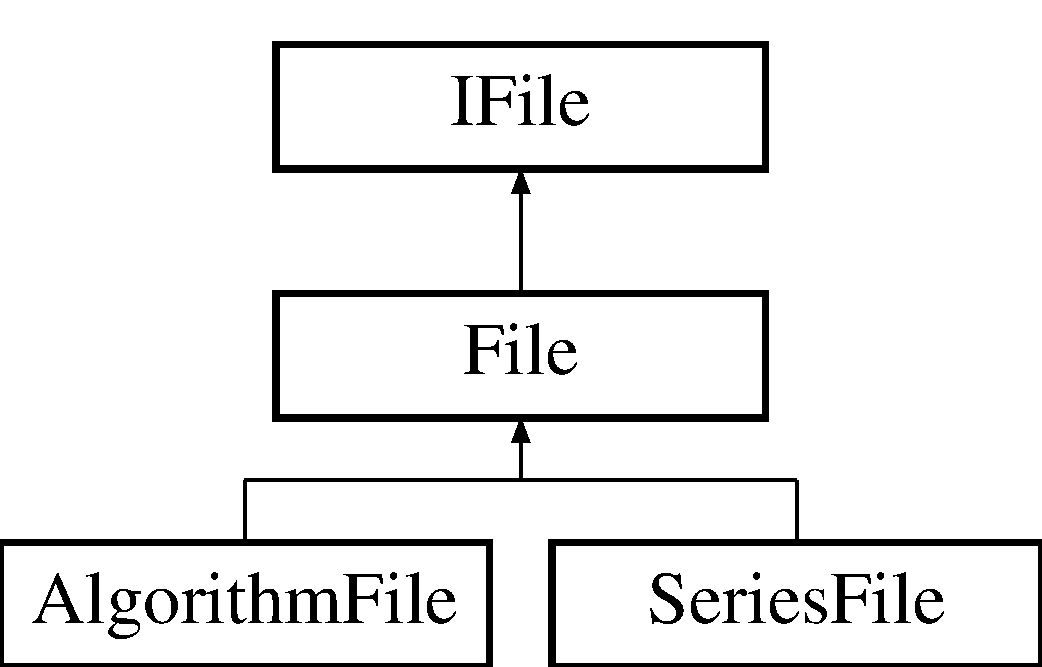
\includegraphics[height=3.000000cm]{class_i_file}
\end{center}
\end{figure}


\subsection{Opis szczegółowy}
Klasa \hyperlink{class_i_file}{I\+File} -\/ interfejs dla różnych plików. 

Dokumentacja dla tej klasy została wygenerowana z plików\+:\begin{DoxyCompactItemize}
\item 
C\+:/\+Users/\+Marcin/\+Desktop/\+Snakes\+\_\+snakes/ifile.\+h\item 
C\+:/\+Users/\+Marcin/\+Desktop/\+Snakes\+\_\+snakes/ifile.\+cpp\end{DoxyCompactItemize}

\hypertarget{class_i_interpreter}{\section{Dokumentacja klasy I\+Interpreter}
\label{class_i_interpreter}\index{I\+Interpreter@{I\+Interpreter}}
}


Klasa \hyperlink{class_i_interpreter}{I\+Interpreter} -\/ interfejs dla interpreterów.  




{\ttfamily \#include $<$iinterpreter.\+h$>$}

Diagram dziedziczenia dla I\+Interpreter\begin{figure}[H]
\begin{center}
\leavevmode
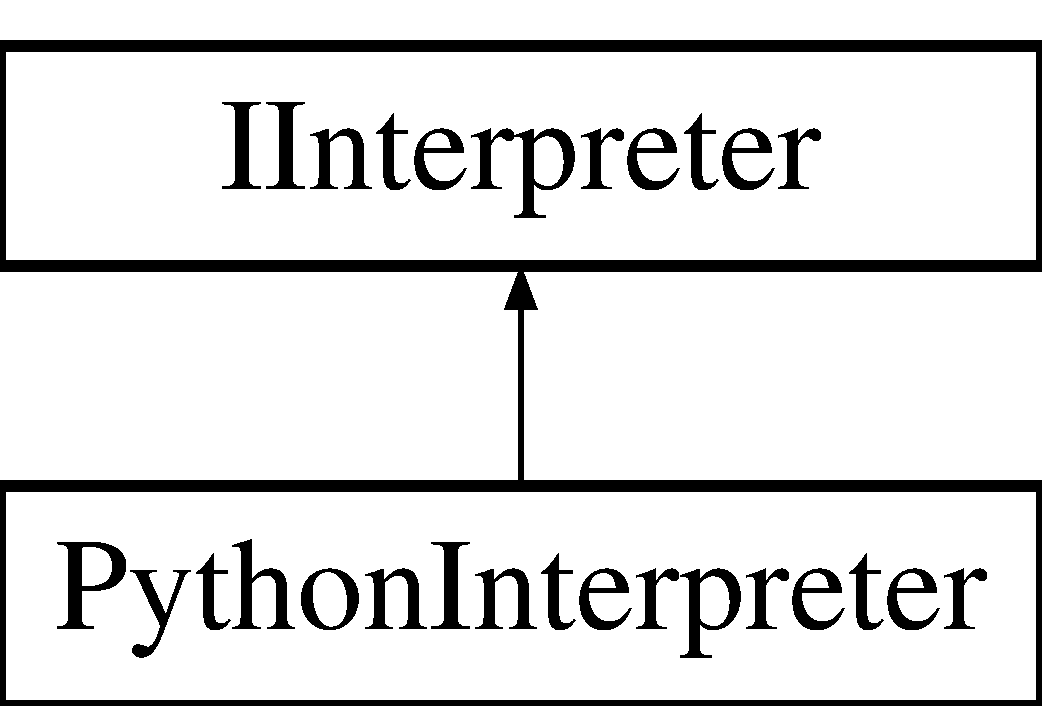
\includegraphics[height=2.000000cm]{class_i_interpreter}
\end{center}
\end{figure}


\subsection{Opis szczegółowy}
Klasa \hyperlink{class_i_interpreter}{I\+Interpreter} -\/ interfejs dla interpreterów. 

Dokumentacja dla tej klasy została wygenerowana z plików\+:\begin{DoxyCompactItemize}
\item 
C\+:/\+Users/\+Marcin/\+Desktop/\+Snakes\+\_\+snakes/iinterpreter.\+h\item 
C\+:/\+Users/\+Marcin/\+Desktop/\+Snakes\+\_\+snakes/iinterpreter.\+cpp\end{DoxyCompactItemize}

\hypertarget{class_point}{\section{Dokumentacja klasy Point}
\label{class_point}\index{Point@{Point}}
}


Klasa \hyperlink{class_point}{Point} -\/ obiekty tej klasy przechowują informacje o punkcie serii.  




{\ttfamily \#include $<$point.\+h$>$}

\subsection*{Metody publiczne}
\begin{DoxyCompactItemize}
\item 
Q\+Date\+Time \hyperlink{class_point_aee53ff6b0e8d20a149fae879ff7c6e4c}{get\+Time} ()
\begin{DoxyCompactList}\small\item\em get\+Time -\/ metoda pobiera znacznik czasowy punktu \end{DoxyCompactList}\item 
void \hyperlink{class_point_a930173774856f75664596a84c9b72c3f}{set\+Time} (Q\+Date\+Time \+\_\+time)
\begin{DoxyCompactList}\small\item\em set\+Time -\/ metoda ustawia znacznik czasowy punktu \end{DoxyCompactList}\item 
double \hyperlink{class_point_ae63f2e3c115c31681526d8f5f8620c0f}{get\+Value} ()
\begin{DoxyCompactList}\small\item\em get\+Value -\/ metoda pobiera wartość punktu \end{DoxyCompactList}\item 
void \hyperlink{class_point_a048c1d16cb855b4989454331dcd42e19}{set\+Value} (double \+\_\+value)
\begin{DoxyCompactList}\small\item\em set\+Value -\/ metoda ustawia wartość punktu \end{DoxyCompactList}\item 
double \hyperlink{class_point_a7337f6e918f0e33c67517f02d9b0125c}{get\+Reliability} ()
\begin{DoxyCompactList}\small\item\em get\+Reliability -\/ metoda pobiera wiarygodność punktu \end{DoxyCompactList}\item 
void \hyperlink{class_point_a123692f9126c70a9e436a1a60bc86213}{set\+Reliability} (double \+\_\+reliability)
\begin{DoxyCompactList}\small\item\em set\+Reliability -\/ metoda ustawia wiarygodność punktu \end{DoxyCompactList}\end{DoxyCompactItemize}


\subsection{Opis szczegółowy}
Klasa \hyperlink{class_point}{Point} -\/ obiekty tej klasy przechowują informacje o punkcie serii. 

\subsection{Dokumentacja funkcji składowych}
\hypertarget{class_point_a7337f6e918f0e33c67517f02d9b0125c}{\index{Point@{Point}!get\+Reliability@{get\+Reliability}}
\index{get\+Reliability@{get\+Reliability}!Point@{Point}}
\subsubsection[{get\+Reliability}]{\setlength{\rightskip}{0pt plus 5cm}double Point\+::get\+Reliability (
\begin{DoxyParamCaption}
{}
\end{DoxyParamCaption}
)}}\label{class_point_a7337f6e918f0e33c67517f02d9b0125c}


get\+Reliability -\/ metoda pobiera wiarygodność punktu 

\begin{DoxyReturn}{Zwraca}
-\/ wiarygodność punktu 
\end{DoxyReturn}
\hypertarget{class_point_aee53ff6b0e8d20a149fae879ff7c6e4c}{\index{Point@{Point}!get\+Time@{get\+Time}}
\index{get\+Time@{get\+Time}!Point@{Point}}
\subsubsection[{get\+Time}]{\setlength{\rightskip}{0pt plus 5cm}Q\+Date\+Time Point\+::get\+Time (
\begin{DoxyParamCaption}
{}
\end{DoxyParamCaption}
)}}\label{class_point_aee53ff6b0e8d20a149fae879ff7c6e4c}


get\+Time -\/ metoda pobiera znacznik czasowy punktu 

\begin{DoxyReturn}{Zwraca}
-\/ znacznik czasowy punktu 
\end{DoxyReturn}
\hypertarget{class_point_ae63f2e3c115c31681526d8f5f8620c0f}{\index{Point@{Point}!get\+Value@{get\+Value}}
\index{get\+Value@{get\+Value}!Point@{Point}}
\subsubsection[{get\+Value}]{\setlength{\rightskip}{0pt plus 5cm}double Point\+::get\+Value (
\begin{DoxyParamCaption}
{}
\end{DoxyParamCaption}
)}}\label{class_point_ae63f2e3c115c31681526d8f5f8620c0f}


get\+Value -\/ metoda pobiera wartość punktu 

\begin{DoxyReturn}{Zwraca}
-\/ wartość punktu 
\end{DoxyReturn}
\hypertarget{class_point_a123692f9126c70a9e436a1a60bc86213}{\index{Point@{Point}!set\+Reliability@{set\+Reliability}}
\index{set\+Reliability@{set\+Reliability}!Point@{Point}}
\subsubsection[{set\+Reliability}]{\setlength{\rightskip}{0pt plus 5cm}void Point\+::set\+Reliability (
\begin{DoxyParamCaption}
\item[{double}]{\+\_\+reliability}
\end{DoxyParamCaption}
)}}\label{class_point_a123692f9126c70a9e436a1a60bc86213}


set\+Reliability -\/ metoda ustawia wiarygodność punktu 


\begin{DoxyParams}{Parametry}
{\em \+\_\+reliability} & -\/ wiarygodność punktu do ustawienia \\
\hline
\end{DoxyParams}
\hypertarget{class_point_a930173774856f75664596a84c9b72c3f}{\index{Point@{Point}!set\+Time@{set\+Time}}
\index{set\+Time@{set\+Time}!Point@{Point}}
\subsubsection[{set\+Time}]{\setlength{\rightskip}{0pt plus 5cm}void Point\+::set\+Time (
\begin{DoxyParamCaption}
\item[{Q\+Date\+Time}]{\+\_\+time}
\end{DoxyParamCaption}
)}}\label{class_point_a930173774856f75664596a84c9b72c3f}


set\+Time -\/ metoda ustawia znacznik czasowy punktu 


\begin{DoxyParams}{Parametry}
{\em \+\_\+time} & -\/ znacznik czasowy punktu do ustawienia \\
\hline
\end{DoxyParams}
\hypertarget{class_point_a048c1d16cb855b4989454331dcd42e19}{\index{Point@{Point}!set\+Value@{set\+Value}}
\index{set\+Value@{set\+Value}!Point@{Point}}
\subsubsection[{set\+Value}]{\setlength{\rightskip}{0pt plus 5cm}void Point\+::set\+Value (
\begin{DoxyParamCaption}
\item[{double}]{\+\_\+value}
\end{DoxyParamCaption}
)}}\label{class_point_a048c1d16cb855b4989454331dcd42e19}


set\+Value -\/ metoda ustawia wartość punktu 


\begin{DoxyParams}{Parametry}
{\em \+\_\+value} & -\/ wartość punktu do ustawienia \\
\hline
\end{DoxyParams}


Dokumentacja dla tej klasy została wygenerowana z plików\+:\begin{DoxyCompactItemize}
\item 
C\+:/\+Users/\+Marcin/\+Desktop/\+Snakes\+\_\+snakes/point.\+h\item 
C\+:/\+Users/\+Marcin/\+Desktop/\+Snakes\+\_\+snakes/point.\+cpp\end{DoxyCompactItemize}

\hypertarget{class_python_interpreter}{\section{Dokumentacja klasy Python\+Interpreter}
\label{class_python_interpreter}\index{Python\+Interpreter@{Python\+Interpreter}}
}


Klasa \hyperlink{class_python_interpreter}{Python\+Interpreter} -\/ interpreter.  




{\ttfamily \#include $<$pythoninterpreter.\+h$>$}

Diagram dziedziczenia dla Python\+Interpreter\begin{figure}[H]
\begin{center}
\leavevmode
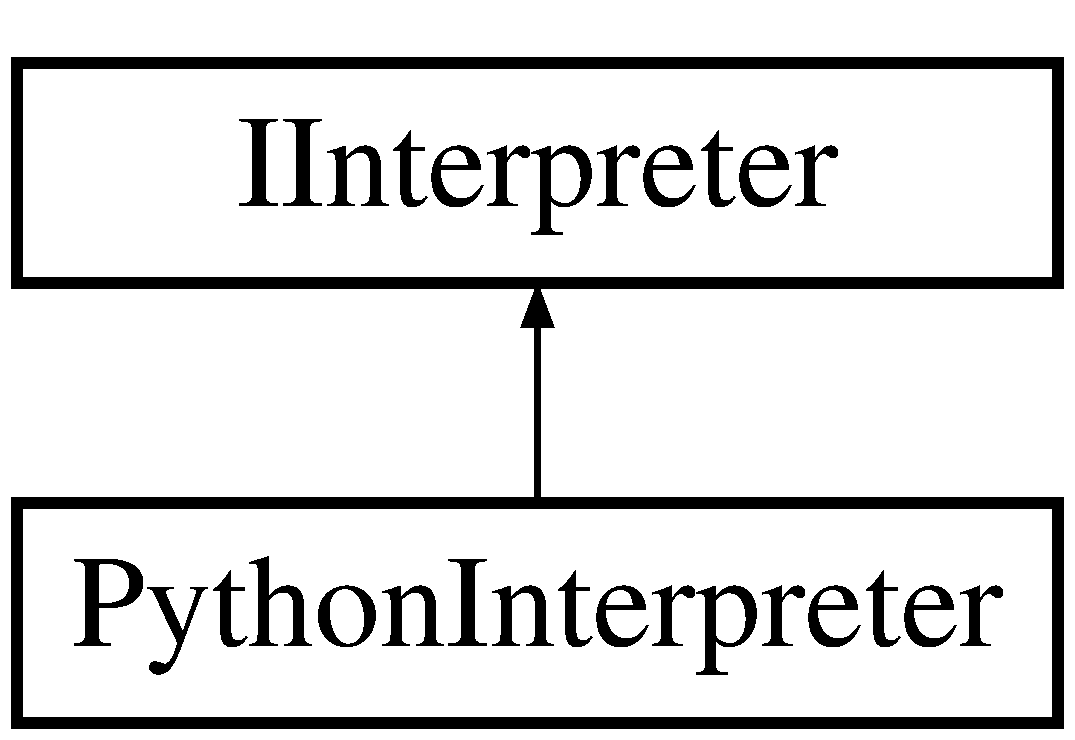
\includegraphics[height=2.000000cm]{class_python_interpreter}
\end{center}
\end{figure}
\subsection*{Metody publiczne}
\begin{DoxyCompactItemize}
\item 
\hypertarget{class_python_interpreter_ae44c1714d8fe0f955369de9f3e5a0e31}{void \hyperlink{class_python_interpreter_ae44c1714d8fe0f955369de9f3e5a0e31}{initialize} ()}\label{class_python_interpreter_ae44c1714d8fe0f955369de9f3e5a0e31}

\begin{DoxyCompactList}\small\item\em initialize -\/ metoda inicjalizuje pracę interpretera \end{DoxyCompactList}\item 
double \hyperlink{class_python_interpreter_a93e0c709989ec0d3cb427dbd77e5a9fb}{execute} (Q\+String \+\_\+script, double \+\_\+input\+Value)
\begin{DoxyCompactList}\small\item\em execute -\/ metoda wywołuje skrypt na wybranej danej \end{DoxyCompactList}\item 
\hypertarget{class_python_interpreter_acdc9d0c1c3231ee74f467cc4d41f891c}{void \hyperlink{class_python_interpreter_acdc9d0c1c3231ee74f467cc4d41f891c}{finalize} ()}\label{class_python_interpreter_acdc9d0c1c3231ee74f467cc4d41f891c}

\begin{DoxyCompactList}\small\item\em finalize -\/ metoda finalizuje działanie interpretera \end{DoxyCompactList}\end{DoxyCompactItemize}


\subsection{Opis szczegółowy}
Klasa \hyperlink{class_python_interpreter}{Python\+Interpreter} -\/ interpreter. 

\subsection{Dokumentacja funkcji składowych}
\hypertarget{class_python_interpreter_a93e0c709989ec0d3cb427dbd77e5a9fb}{\index{Python\+Interpreter@{Python\+Interpreter}!execute@{execute}}
\index{execute@{execute}!Python\+Interpreter@{Python\+Interpreter}}
\subsubsection[{execute}]{\setlength{\rightskip}{0pt plus 5cm}double Python\+Interpreter\+::execute (
\begin{DoxyParamCaption}
\item[{Q\+String}]{\+\_\+script, }
\item[{double}]{\+\_\+input\+Value}
\end{DoxyParamCaption}
)\hspace{0.3cm}{\ttfamily [virtual]}}}\label{class_python_interpreter_a93e0c709989ec0d3cb427dbd77e5a9fb}


execute -\/ metoda wywołuje skrypt na wybranej danej 


\begin{DoxyParams}{Parametry}
{\em \+\_\+script} & -\/ skrypt do wykonania \\
\hline
{\em \+\_\+input\+Value} & -\/ wartość punktu do przetworzenia \\
\hline
\end{DoxyParams}
\begin{DoxyReturn}{Zwraca}

\end{DoxyReturn}


Implementuje \hyperlink{class_i_interpreter}{I\+Interpreter}.



Dokumentacja dla tej klasy została wygenerowana z plików\+:\begin{DoxyCompactItemize}
\item 
C\+:/\+Users/\+Marcin/\+Desktop/\+Snakes\+\_\+snakes/pythoninterpreter.\+h\item 
C\+:/\+Users/\+Marcin/\+Desktop/\+Snakes\+\_\+snakes/pythoninterpreter.\+cpp\end{DoxyCompactItemize}

\hypertarget{class_series}{\section{Dokumentacja klasy Series}
\label{class_series}\index{Series@{Series}}
}


Klasa \hyperlink{class_series}{Series} -\/ obiekt tej klasy przechowuje informacje o serii.  




{\ttfamily \#include $<$series.\+h$>$}

\subsection*{Metody publiczne}
\begin{DoxyCompactItemize}
\item 
Q\+String \hyperlink{class_series_aeec7b0318147f133101233930a9fe0bd}{get\+Name} ()
\begin{DoxyCompactList}\small\item\em get\+Name -\/ metoda pobiera nazwę serii \end{DoxyCompactList}\item 
void \hyperlink{class_series_a45e36a2f91ffda781a2bd6ac1e42799a}{set\+Name} (Q\+String \+\_\+name)
\begin{DoxyCompactList}\small\item\em set\+Name -\/ metoda ustawia nazwę serii \end{DoxyCompactList}\item 
std\+::vector$<$ \hyperlink{class_point}{Point} $>$ \hyperlink{class_series_acce7f1886fd9fca8a0bed0de308d3206}{get\+Points} ()
\begin{DoxyCompactList}\small\item\em get\+Points -\/ metoda pobiera punkty wchodzące w skład serii \end{DoxyCompactList}\item 
void \hyperlink{class_series_ae1c659538591e22f42495c281934e2a3}{set\+Points} (std\+::vector$<$ \hyperlink{class_point}{Point} $>$ \+\_\+points)
\begin{DoxyCompactList}\small\item\em set\+Points -\/ metoda ustawia punkty dla serii \end{DoxyCompactList}\item 
void \hyperlink{class_series_aedcbd470ac2ae2807be45c2339503991}{add\+Point} (Q\+Date\+Time \+\_\+time, double \+\_\+value, double \+\_\+reliability)
\begin{DoxyCompactList}\small\item\em add\+Point -\/ metoda służy do dodawania punktów dla serii \end{DoxyCompactList}\end{DoxyCompactItemize}
\subsection*{Statyczne metody publiczne}
\begin{DoxyCompactItemize}
\item 
static \hyperlink{class_series}{Series} $\ast$ \hyperlink{class_series_ab8c7554def83d47ed71333b48e2b7bd2}{copy} (\hyperlink{class_series}{Series} $\ast$\+\_\+series)
\begin{DoxyCompactList}\small\item\em copy -\/ metoda kopiuje serię (kopiowanie głębokie) \end{DoxyCompactList}\end{DoxyCompactItemize}


\subsection{Opis szczegółowy}
Klasa \hyperlink{class_series}{Series} -\/ obiekt tej klasy przechowuje informacje o serii. 

\subsection{Dokumentacja funkcji składowych}
\hypertarget{class_series_aedcbd470ac2ae2807be45c2339503991}{\index{Series@{Series}!add\+Point@{add\+Point}}
\index{add\+Point@{add\+Point}!Series@{Series}}
\subsubsection[{add\+Point}]{\setlength{\rightskip}{0pt plus 5cm}void Series\+::add\+Point (
\begin{DoxyParamCaption}
\item[{Q\+Date\+Time}]{\+\_\+time, }
\item[{double}]{\+\_\+value, }
\item[{double}]{\+\_\+reliability}
\end{DoxyParamCaption}
)}}\label{class_series_aedcbd470ac2ae2807be45c2339503991}


add\+Point -\/ metoda służy do dodawania punktów dla serii 


\begin{DoxyParams}{Parametry}
{\em \+\_\+time} & -\/ znacznik czasowy nowego punktu w serii \\
\hline
{\em \+\_\+value} & -\/ wartość pomiaru nowego punktu w serii \\
\hline
{\em \+\_\+reliability} & -\/ wiarygodność nowego punktu w serii \\
\hline
\end{DoxyParams}
\hypertarget{class_series_ab8c7554def83d47ed71333b48e2b7bd2}{\index{Series@{Series}!copy@{copy}}
\index{copy@{copy}!Series@{Series}}
\subsubsection[{copy}]{\setlength{\rightskip}{0pt plus 5cm}{\bf Series} $\ast$ Series\+::copy (
\begin{DoxyParamCaption}
\item[{{\bf Series} $\ast$}]{\+\_\+series}
\end{DoxyParamCaption}
)\hspace{0.3cm}{\ttfamily [static]}}}\label{class_series_ab8c7554def83d47ed71333b48e2b7bd2}


copy -\/ metoda kopiuje serię (kopiowanie głębokie) 


\begin{DoxyParams}{Parametry}
{\em \+\_\+series} & -\/ seria do skopiowania \\
\hline
\end{DoxyParams}
\begin{DoxyReturn}{Zwraca}
-\/ wskaźnik na nową serię 
\end{DoxyReturn}
\hypertarget{class_series_aeec7b0318147f133101233930a9fe0bd}{\index{Series@{Series}!get\+Name@{get\+Name}}
\index{get\+Name@{get\+Name}!Series@{Series}}
\subsubsection[{get\+Name}]{\setlength{\rightskip}{0pt plus 5cm}Q\+String Series\+::get\+Name (
\begin{DoxyParamCaption}
{}
\end{DoxyParamCaption}
)}}\label{class_series_aeec7b0318147f133101233930a9fe0bd}


get\+Name -\/ metoda pobiera nazwę serii 

\begin{DoxyReturn}{Zwraca}
-\/ nazwa serii 
\end{DoxyReturn}
\hypertarget{class_series_acce7f1886fd9fca8a0bed0de308d3206}{\index{Series@{Series}!get\+Points@{get\+Points}}
\index{get\+Points@{get\+Points}!Series@{Series}}
\subsubsection[{get\+Points}]{\setlength{\rightskip}{0pt plus 5cm}std\+::vector$<$ {\bf Point} $>$ Series\+::get\+Points (
\begin{DoxyParamCaption}
{}
\end{DoxyParamCaption}
)}}\label{class_series_acce7f1886fd9fca8a0bed0de308d3206}


get\+Points -\/ metoda pobiera punkty wchodzące w skład serii 

\begin{DoxyReturn}{Zwraca}
-\/ wektor punktów wchodzących w skład serii 
\end{DoxyReturn}
\hypertarget{class_series_a45e36a2f91ffda781a2bd6ac1e42799a}{\index{Series@{Series}!set\+Name@{set\+Name}}
\index{set\+Name@{set\+Name}!Series@{Series}}
\subsubsection[{set\+Name}]{\setlength{\rightskip}{0pt plus 5cm}void Series\+::set\+Name (
\begin{DoxyParamCaption}
\item[{Q\+String}]{\+\_\+name}
\end{DoxyParamCaption}
)}}\label{class_series_a45e36a2f91ffda781a2bd6ac1e42799a}


set\+Name -\/ metoda ustawia nazwę serii 


\begin{DoxyParams}{Parametry}
{\em \+\_\+name} & -\/ nazwa serii do ustawienia \\
\hline
\end{DoxyParams}
\hypertarget{class_series_ae1c659538591e22f42495c281934e2a3}{\index{Series@{Series}!set\+Points@{set\+Points}}
\index{set\+Points@{set\+Points}!Series@{Series}}
\subsubsection[{set\+Points}]{\setlength{\rightskip}{0pt plus 5cm}void Series\+::set\+Points (
\begin{DoxyParamCaption}
\item[{std\+::vector$<$ {\bf Point} $>$}]{\+\_\+points}
\end{DoxyParamCaption}
)}}\label{class_series_ae1c659538591e22f42495c281934e2a3}


set\+Points -\/ metoda ustawia punkty dla serii 


\begin{DoxyParams}{Parametry}
{\em \+\_\+points} & -\/ punkty do ustawienia \\
\hline
\end{DoxyParams}


Dokumentacja dla tej klasy została wygenerowana z plików\+:\begin{DoxyCompactItemize}
\item 
C\+:/\+Users/\+Marcin/\+Desktop/\+Snakes\+\_\+snakes/series.\+h\item 
C\+:/\+Users/\+Marcin/\+Desktop/\+Snakes\+\_\+snakes/series.\+cpp\end{DoxyCompactItemize}

\hypertarget{class_series_file}{\section{Dokumentacja klasy Series\+File}
\label{class_series_file}\index{Series\+File@{Series\+File}}
}


Klasa \hyperlink{class_series_file}{Series\+File} -\/ obiekty tej klasy przechowują informacje o pliku z którego jest wczytywana seria.  




{\ttfamily \#include $<$seriesfile.\+h$>$}

Diagram dziedziczenia dla Series\+File\begin{figure}[H]
\begin{center}
\leavevmode
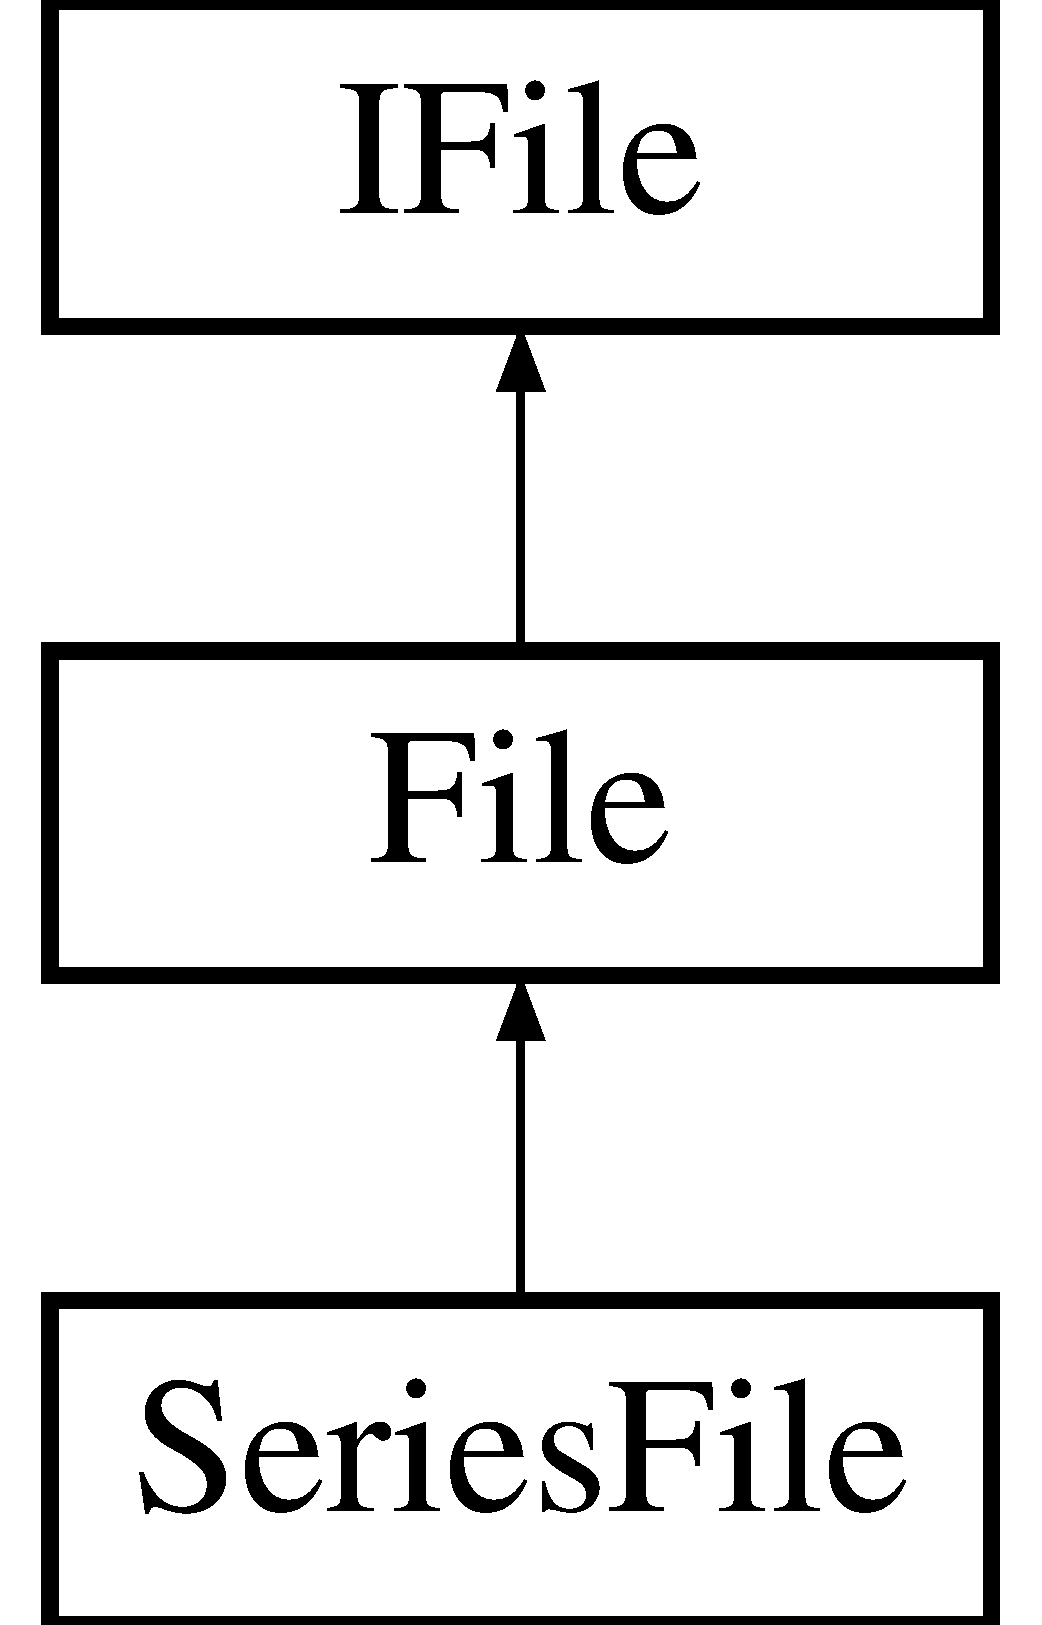
\includegraphics[height=3.000000cm]{class_series_file}
\end{center}
\end{figure}
\subsection*{Metody publiczne}
\begin{DoxyCompactItemize}
\item 
Q\+String\+List \hyperlink{class_series_file_a343a10077b14bade1a98ae69fd47e3a9}{prepare\+Content\+To\+Set} ()
\begin{DoxyCompactList}\small\item\em prepare\+Content\+To\+Set -\/ metoda przygotowuje zawartość pliku dla pól obiektu klasy \hyperlink{class_series}{Series} \end{DoxyCompactList}\item 
Q\+String \hyperlink{class_series_file_a2837d5d09c7f9014852370b120b9ba81}{prepare\+Content\+To\+Save} (\hyperlink{class_data_manager}{Data\+Manager} \&\+\_\+data\+Manger, char c)
\begin{DoxyCompactList}\small\item\em prepare\+Content\+To\+Save -\/ metoda przygotowuje skrypt do zapisu w pliu \end{DoxyCompactList}\end{DoxyCompactItemize}
\subsection*{Dodatkowe Dziedziczone Składowe}


\subsection{Opis szczegółowy}
Klasa \hyperlink{class_series_file}{Series\+File} -\/ obiekty tej klasy przechowują informacje o pliku z którego jest wczytywana seria. 

\subsection{Dokumentacja funkcji składowych}
\hypertarget{class_series_file_a2837d5d09c7f9014852370b120b9ba81}{\index{Series\+File@{Series\+File}!prepare\+Content\+To\+Save@{prepare\+Content\+To\+Save}}
\index{prepare\+Content\+To\+Save@{prepare\+Content\+To\+Save}!Series\+File@{Series\+File}}
\subsubsection[{prepare\+Content\+To\+Save}]{\setlength{\rightskip}{0pt plus 5cm}Q\+String Series\+File\+::prepare\+Content\+To\+Save (
\begin{DoxyParamCaption}
\item[{{\bf Data\+Manager} \&}]{\+\_\+data\+Manger, }
\item[{char}]{c}
\end{DoxyParamCaption}
)\hspace{0.3cm}{\ttfamily [virtual]}}}\label{class_series_file_a2837d5d09c7f9014852370b120b9ba81}


prepare\+Content\+To\+Save -\/ metoda przygotowuje skrypt do zapisu w pliu 


\begin{DoxyParams}{Parametry}
{\em \+\_\+data\+Manger} & -\/ parametr niezbędny do pobrania informacji o aktualnie wybranej serii \\
\hline
{\em c} & -\/ parametr informujący o tym co będzie zapisane \\
\hline
\end{DoxyParams}
\begin{DoxyReturn}{Zwraca}
-\/ przygotowana treść do zapisu 
\end{DoxyReturn}


Implementuje \hyperlink{class_file}{File}.

\hypertarget{class_series_file_a343a10077b14bade1a98ae69fd47e3a9}{\index{Series\+File@{Series\+File}!prepare\+Content\+To\+Set@{prepare\+Content\+To\+Set}}
\index{prepare\+Content\+To\+Set@{prepare\+Content\+To\+Set}!Series\+File@{Series\+File}}
\subsubsection[{prepare\+Content\+To\+Set}]{\setlength{\rightskip}{0pt plus 5cm}Q\+String\+List Series\+File\+::prepare\+Content\+To\+Set (
\begin{DoxyParamCaption}
{}
\end{DoxyParamCaption}
)\hspace{0.3cm}{\ttfamily [virtual]}}}\label{class_series_file_a343a10077b14bade1a98ae69fd47e3a9}


prepare\+Content\+To\+Set -\/ metoda przygotowuje zawartość pliku dla pól obiektu klasy \hyperlink{class_series}{Series} 

\begin{DoxyReturn}{Zwraca}
-\/ przygotowana treść do ustawienia w obiecie klasy \hyperlink{class_series}{Series} 
\end{DoxyReturn}


Implementuje \hyperlink{class_file}{File}.



Dokumentacja dla tej klasy została wygenerowana z plików\+:\begin{DoxyCompactItemize}
\item 
C\+:/\+Users/\+Marcin/\+Desktop/\+Snakes\+\_\+snakes/seriesfile.\+h\item 
C\+:/\+Users/\+Marcin/\+Desktop/\+Snakes\+\_\+snakes/seriesfile.\+cpp\end{DoxyCompactItemize}

%--- End generated contents ---

% Index
\newpage
\phantomsection
\addcontentsline{toc}{chapter}{Indeks}
\printindex

\end{document}
